\documentclass[a4paper,12pt]{article}
\usepackage[utf8x]{inputenc}
\usepackage{graphicx}
%\usepackage{epstopdf}
%\usepackage{phdthesis}
\usepackage{euler}
\usepackage{palatino}
\usepackage{listings}
\usepackage{tikz} 
%opening
\title{Tutorial 1. Introduction to MOA \\ \{M\}assive \{O\}nline \{A\}nalysis}
\author{Albert Bifet and Richard Kirkby}
\date{March 2012}

\newtheorem{definition}{Definition}{}
\newtheorem{exercise}{Exercise}{}

\begin{document}
\lstset{language=Java,basicstyle=\tiny,numbers=left}
\maketitle
\begin{center}

\includegraphics[height=3cm]{images/LogoMOA.jpg} \\

\includegraphics[height=4cm]{images/Waikato.jpg} \\ 
\end{center}
\thispagestyle{empty}
\newpage
\setcounter{page}{1}

\section{Getting Started}

This tutorial is a basic introduction to MOA.
{\bf M}assive {\bf O}nline {\bf A}nalysis (MOA) is a  
software environment for implementing algorithms and running experiments
for online learning from 
evolving data streams.

%\begin{center}
\includegraphics[height=2cm]{LogoMOA.jpg} \end{center}

%MOA includes a collection of classification and clustering methods as well as tools for evaluation. 
We suppose that MOA is installed in your system.
Start a graphical user interface for configuring and running tasks with the command:

\begin{verbatim}
java -cp moa.jar -javaagent:sizeofag.jar moa.gui.GUI
\end{verbatim}

\begin{figure}[h]
\begin{center} 
%\epsfig{file=MOA_Task.ps, scale=0.3}
%\epsfig{file=Configure_task.ps, scale=0.33}
\includegraphics[height=2.5in]{images/MOA_Task.png}%{MOATask.png}
%\includegraphics[height=2.5in]{Configure_task.pdf}
\end{center} 
\caption{MOA Graphical User Interface}
\label{fig:moagui}
\end{figure}

Click 'Configure' to set up a task, when ready click to launch a task click 'Run'. Several tasks can be run concurrently. 
Click on different tasks in the list and control them using the buttons below.
 If textual output of a task is available it will be displayed in the middle of the GUI, and can be saved to disk.

Note that the command line text box displayed at the top of the window represents textual commands that can be used to run tasks on the command line.
 The text can be selected then copied onto the clipboard. In the bottom of the GUI there is a graphical display of the results. It is possible
to compare the results of two different tasks: the current task is displayed in red, and the selected previously is in blue. 


%The classification GUI of MOA is divided in five parts:
%\begin{itemize}
% \item Configuration line where the tasks to run are specified
% \item List of Tasks running or finished
% \item Buttons to pause, resume, cancel or delete tasks
% \item Task result output
% \item Button to export the task results in a file
%\end{itemize}

\section{The Classification Graphical User Interface}

We start comparing the accuracy of two classifiers. First, we explain briefly two different data stream evaluations.% have to decide which data stream evaluation to use.

\subsection{Data streams Evaluation}
The most significant requirements for a data stream setting are the following: 
\begin{description}
\item[Requirement 1] Process an example at a time, and inspect
 it only once (at most)
\item[Requirement 2] Use a limited amount of memory
\item[Requirement 3] Work in a limited amount of time
\item[Requirement 4] Be ready to predict at any time
\end{description}
\begin{figure}[t]
\begin{center} 
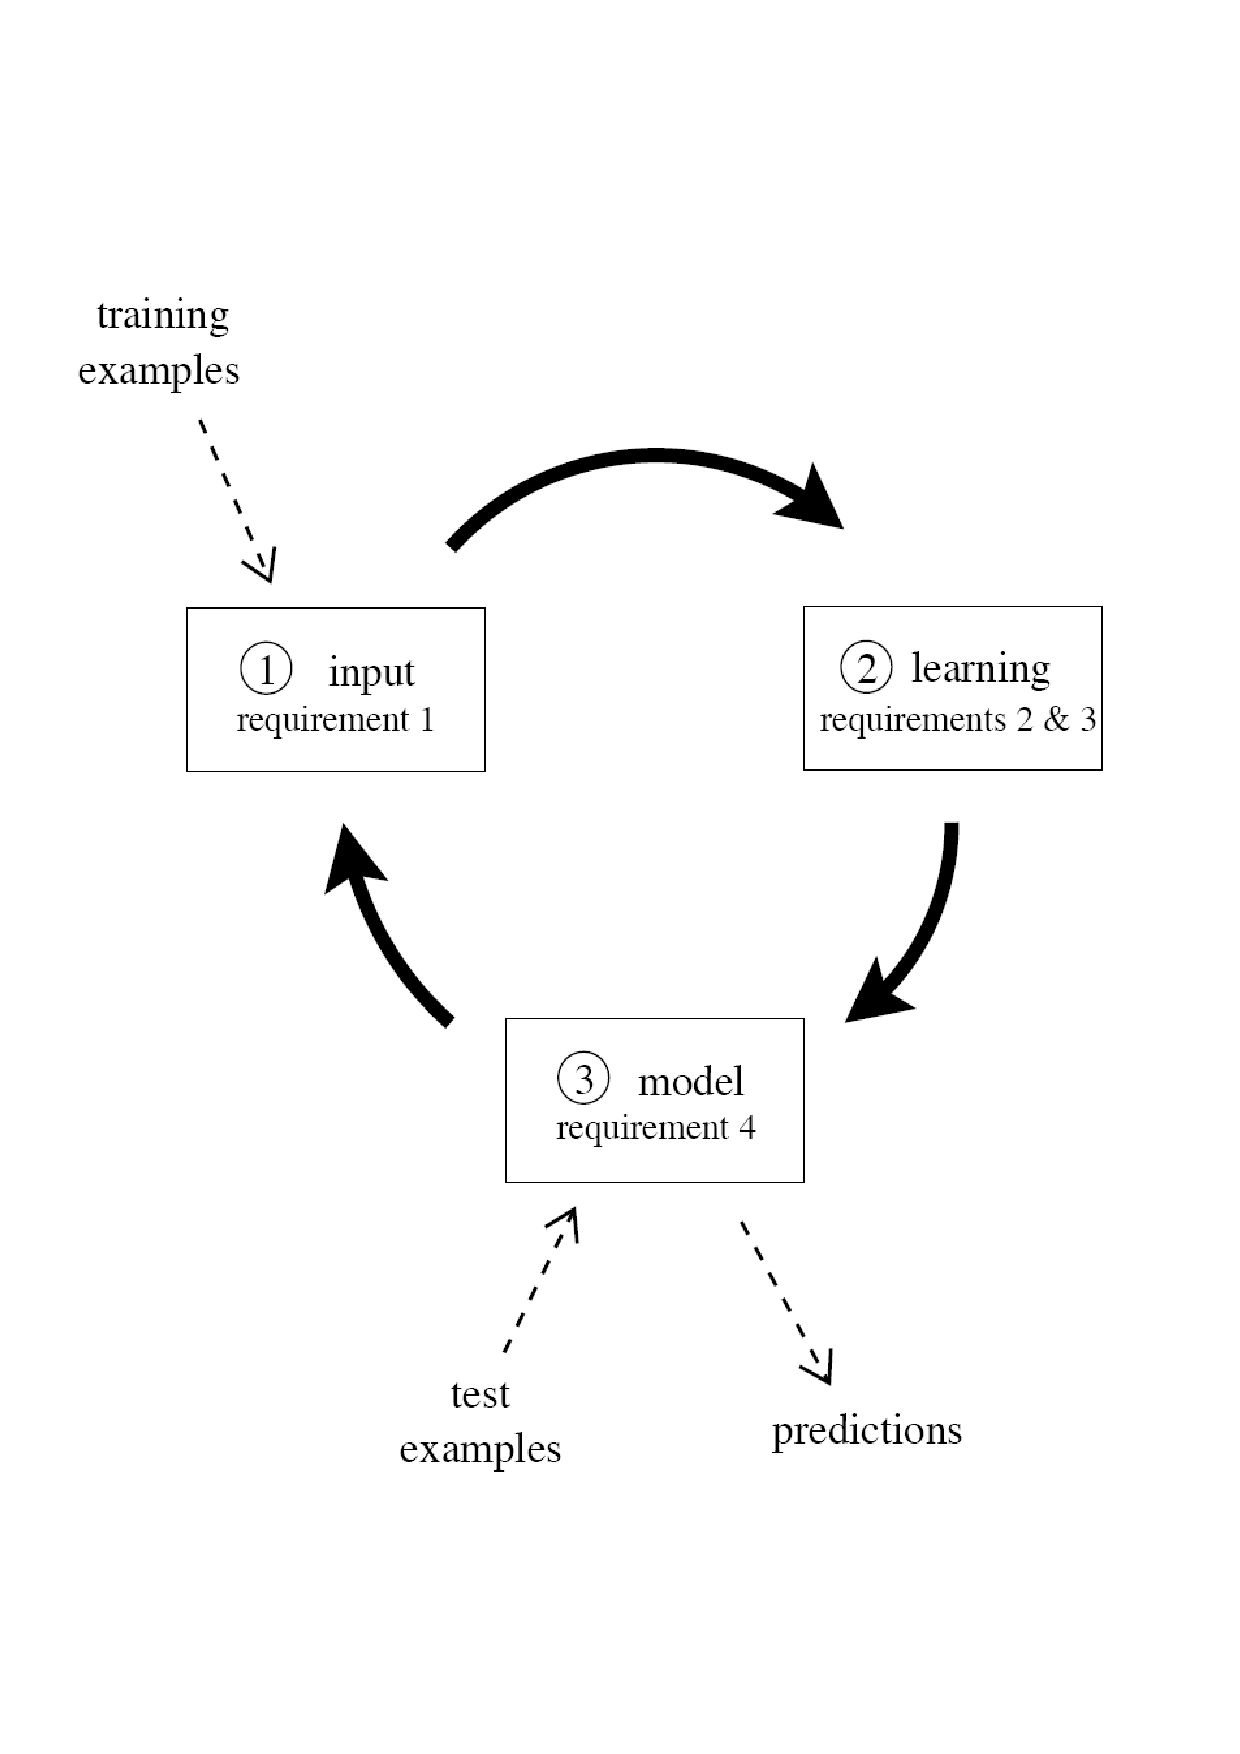
\includegraphics[height=9cm]{images/Frame.pdf}
\end{center} 
\caption{The data stream classification cycle}
\label{fig:cycle}
\end{figure} 

Figure~\ref{fig:cycle} illustrates the typical use of a data stream 
classification algorithm, and how the requirements fit 
in a repeating cycle:
\begin{enumerate}
\item  The algorithm is passed the next available example from the stream
   (requirement 1).
\item  The algorithm processes the example, updating its data structures. It
   does so without exceeding the memory bounds set on it (requirement 2),
   and as quickly as possible (requirement 3).
\item  The algorithm is ready to accept the next example. On request it is
   able to predict the class of unseen examples
   % , and  supply a model that can be used to  
   (requirement 4).
\end{enumerate}

In traditional batch learning the problem of limited data is overcome
by analyzing and averaging multiple models produced with different random
arrangements of training and test data. In the stream setting the problem of
(effectively) unlimited data poses different challenges. One solution involves
taking snapshots at different times during the induction of a model to see how
much the model improves.

%The evaluation procedure of a learning algorithm determines which examples
%are used for training the algorithm, and which are used to test the model output
%by the algorithm. The procedure used historically in batch learning has partly
%depended on data size. As data sizes increase, practical
%time limitations prevent procedures that repeat training too many times. It is
%commonly accepted with considerably larger data sources that it is necessary
%to reduce the numbers of repetitions or folds to allow experiments to complete
%in reasonable time. 
    When considering what procedure to use in the data stream setting, one of
the unique concerns is how to build a picture of accuracy over time. Two main
approaches arise:
\begin{itemize}
 \item {\bf Holdout}:
When traditional batch learning reaches a scale where cross-validation is too time 
consuming, it is often accepted to instead measure performance on a single holdout
set. This is most useful when the division between train and test sets have
been pre-defined, so that results from different studies can be directly compared. 
\item {\bf Interleaved Test-Then-Train or Prequential}:
 Each individual example can be used to test the model
before it is used for training, and from this the accuracy can be incrementally
updated. When intentionally performed in this order, the model is always
being tested on examples it has not seen. This scheme has the advantage that
no holdout set is needed for testing, making maximum use of the available
data. It also ensures a smooth plot of accuracy over time, as each individual
example will become increasingly less significant to the overall average.
\end{itemize}
   
Holdout evaluation gives a more accurate estimation of the accuracy of the classifier on more recent data. However, it requires recent test data that it is difficult to obtain for real datasets.
Gama et al. 
propose to use a forgetting mechanism for estimating holdout accuracy using
prequential
accuracy: a sliding window of size $w$ with the most recent
observations, or fading factors that weigh observations using a decay
factor $\alpha$. 
The output of the two mechanisms is very
similar (every window of size $w_0$ may be approximated by some decay
factor $\alpha_0$).

As data stream classification is a relatively new field, such evaluation 
practices are not nearly as well researched and established as they are
in the traditional batch setting. 


\subsection{Exercises}

To familiarize yourself with the functions discussed so far, please do the following
two exercises. The solutions to these and other exercises in this tutorial are given
at the end.

%\begin{description}
%\item[Exercise 1.] 
\begin{exercise}
Compare the accuracy of the Hoeffding Tree with the Naive Bayes classifier, for a RandomTreeGenerator stream of 1,000,000 instances using Interleaved Test-Then-Train evaluation.
Use for all exercises a sample frequency of $10,000$.
\end{exercise}
%\item[Exercise 2.]
\begin{exercise}
Compare and discuss the accuracy for the same stream of the previous exercise using three different evaluations with a Hoeffding Tree:
\begin{itemize}
 \item Periodic Held Out with 1,000 instances for testing
 \item Interleaved Test Then Train
 \item Prequential with a sliding window of 1,000 instances.
\end{itemize}
\end{exercise}

%\end{description}

\subsection{Drift Stream Generators}

MOA streams are build using generators, reading ARFF files, joining several streams, or filtering streams.
MOA streams generators allow to simulate potentially infinite sequence of data.

Two streams evolving on time are:
\begin{itemize}
\item Rotating Hyperplane
\item Random RBF Generator
\end{itemize}

To model concept drift we only have to set up the drift parameter of the stream. 

We can model concept drift also joining several streams.
%Considering data streams as data generated from pure distributions,
MOA models
a concept drift {event} as a weighted combination %a mixture distribution, 
of two pure distributions that characterizes the target concepts before and after
the drift.  MOA uses 
the sigmoid function, as an elegant and practical solution to define the probability that every new 
instance of the stream belongs to the new concept after the drift.

\begin{figure}
\begin{tikzpicture}[domain=-2:9]
  \draw[step=2,very thin,color=gray] (-0.1,-0.1) grid (8.2,4.2);
  \draw[->] (-2.2,0) -- (8.2,0) node[right] {$t$};
  \draw[->] (0,-0.2) -- (0,4.2) node[above] {$f(t)$};
  \draw[<->] (2,-0.6) -- (6,-0.6) node[below] {};
  \draw[color=blue!50!black, domain=2:6] plot[id=x]   function{(x-2)}           node[right]{}; %{$f(x) =x$};
  %\draw[color=blue]   plot[id=sin] function{sin(x)}       node[right] {$f(x) = \sin x$};
  \draw[color=red!50!black] plot[id=exp] function{4/(1+exp(4-x))} node[right] {$f(t)$};% = 1/{(1+ \mathrm e^{-s (x-x_0)}})$};
  %\shadedraw[left color=gray,right color=green, draw=green!50!black] (2,0) -- (2.5,0) arc (0:45:.5) -- cycle; 
  \colorlet{anglecolor}{blue!50!black}
  \filldraw[fill=blue!20,draw=anglecolor] (2,0) -- (2.5,0) arc(0:45:.5);
  \draw (2.7,.3) node[anglecolor] {$\alpha$};
  \filldraw[fill=blue!20,draw=anglecolor] (4,2) -- (4.5,2) arc(0:45:.5);
  \draw (4.7,2.3) node[anglecolor] {$\alpha$};

  \draw (4,-0.3) node[] {$t_0$};
  \draw (4,-0.9) node[] {$W$};
  \draw (-0.5,2) node[] {$0.5$};
  \draw (-0.5,4) node[] {$1$};

\end{tikzpicture}
\caption{A sigmoid function $f(t) = 1/{(1+ \mathrm e^{-s (t-t_0)}})$.}
\label{fig:ConceptChange}
\end{figure}

We see from Figure~\ref{fig:ConceptChange} that the sigmoid function 
$$f(t) = 1/{(1+ \mathrm e^{-s (t-t_0)}})$$
has a derivative at the point $t_0$ equal to $f'(t_0) = s/4$. The tangent of angle 
$\alpha$ is equal to this derivative, $\tan \alpha = s/4$. We observe that 
$ \tan \alpha = 1/ W$,
and as $s= 4 \tan \alpha$ then $s=4/W$. So the parameter $s$ in the sigmoid 
gives the length of $W$ and the angle $\alpha$. 
In this sigmoid model we only need to specify two parameters : 
$t_0$ the point of change, and $W$ the length of change.
Note that for any positive real number $\beta$ $$f(t_0+\beta \cdot W)=1 -f(t_0-\beta \cdot W),$$ and  that $f(t_0+\beta \cdot W)$ and $f(t_0-\beta \cdot W)$ 
are constant values that don't depend on $t_0$ and $W$: 
$$f(t_0+W/2) = 1 - f(t_0-W/2) = 1/( 1+ e^{-2}) \approx 88.08 \%$$  
$$f(t_0+W) = 1 - f(t_0-W) = 1/( 1+ e^{-4}) \approx 98.20 \%$$  
$$f(t_0+2W) = 1 - f(t_0-2W) = 1/( 1+ e^{-8}) \approx 99.97 \%$$

\begin{definition} %{\bf ($\oplus$-operation)}\\
Given two data streams $a$, $b$, we define $c = a  \oplus^{W}_{t_0} b$ as the 
data stream built joining the two data streams $a$ and $b$, where
$t_0$ is the point of change, $W$ is the length of change and 
\begin{itemize}
 \item $\Pr[ c(t) = a(t)] = \mathrm e^{-4(t-t_0)/W}/{(1+ \mathrm e^{-4(t-t_0)/W})}$
 \item $\Pr[ c(t) = b(t)] = 1/{(1+ \mathrm e^{-4(t-t_0)/W})}$.
\end{itemize}
\end{definition}


Example:
\begin{footnotesize}\begin{verbatim}
 ConceptDriftStream -s (generators.AgrawalGenerator -f 7) 
    -d (generators.AgrawalGenerator -f 2) -w 1000000 -p 900000 
\end{verbatim}\end{footnotesize}
\texttt{ConceptDriftStream} parameters:

\begin{itemize}
\item -s : Stream 
\item -d : Concept drift Stream
\item -p : Central position of concept drift change
\item -w : Width of concept drift change\end{itemize}


\subsection{Exercises}

%\begin{description}
%\item[Exercise 3.] 
\begin{exercise}Compare the accuracy of the Hoeffding Tree with the Naive Bayes classifier, for a RandomRBFGenerator stream of 1,000,000 instances with speed change of 0,001 using Interleaved Test-Then-Train evaluation.  
\end{exercise}
%\item[Exercise 4.] 
\begin{exercise}Compare the accuracy for the same stream of the previous exercise using three different classifiers:
\begin{itemize}
 %\item Majority Class
 \item Hoeffding Tree with Majority Class at the leaves
 \item Hoeffding Adaptive Tree
 \item OzaBagAdwin with 10 HoeffdingTree

\end{itemize}
\end{exercise}


%\end{description}


\section{Using the command line}

An easy way to use the command line, is to copy and paste the text in the Configuration line of the Graphical User Interface.% at the end of

%\begin{verbatim}
%java -cp moa.jar -javaagent:sizeofag.jar moa.DoTask 
%\end{verbatim}

For example, suppose we want to process the task 
\begin{verbatim}EvaluatePrequential -l trees.HoeffdingTree -i 1000000 -w 10000\end{verbatim} 
using the command line. We simply write 
\begin{verbatim}
java -cp moa.jar -javaagent:sizeofag.jar moa.DoTask  \
"EvaluatePrequential -l trees.HoeffdingTree -i 1000000 -w 10000"
\end{verbatim}

Note that some parameters are missing, since they use default values.


\subsection{Learning and Evaluating Models}

%The first example will command MOA to train the \verb+HoeffdingTree+ classifier and create a model.
The \verb+moa.DoTask+ class is the main class for running tasks on the command line. It will accept the name of a task followed by any appropriate parameters. The first task used is the \verb+LearnModel+ task. The \verb+-l+ parameter specifies the learner, in this case the \verb+HoeffdingTree+ class. The \verb+-s+ parameter specifies the stream to learn from, in this case {\tt generators.Wave- formGenerator} is specified, which is a data stream generator that produces a three-class learning problem of identifying three types of waveform. The \verb+-m+ option specifies the maximum number of examples to train the learner with, in this case one million examples. The \verb+-O+ option specifies a file to output the resulting model to:

\begin{verbatim}
java -cp moa.jar -javaagent:sizeofag.jar moa.DoTask \
  LearnModel -l trees.HoeffdingTree \
  -s generators.WaveformGenerator -m 1000000 -O model1.moa
\end{verbatim}

This will create a file named \verb+model1.moa+ that contains the decision stump model that was induced during training.

The next example will evaluate the model to see how accurate it is on a set of examples that are generated using a different random seed. The \verb+EvaluateModel+ task is given the parameters needed to load the model produced in the previous step, generate a new waveform stream with a random seed of 2, and test on one million examples:

\begin{verbatim}
java -cp moa.jar -javaagent:sizeofag.jar moa.DoTask \
  "EvaluateModel -m file:model1.moa \
  -s (generators.WaveformGenerator -i 2) -i 1000000"
\end{verbatim}

This is the first example of nesting parameters using brackets. Quotes have been added around the description of the task, otherwise the operating system may be confused about the meaning of the brackets.

After evaluation the following statistics are output:

\begin{verbatim}
classified instances = 1,000,000
classifications correct (percent) = 84.474
Kappa Statistic (percent) = 76.711
\end{verbatim}

Note the the above two steps can be achieved by rolling them into one, avoiding the need to create an external file, as follows:

\begin{verbatim}
java -cp moa.jar -javaagent:sizeofag.jar moa.DoTask \
  "EvaluateModel -m (LearnModel -l trees.HoeffdingTree \
  -s generators.WaveformGenerator -m 1000000) \
  -s (generators.WaveformGenerator -i 2) -i 1000000"
\end{verbatim}

The task \verb+EvaluatePeriodicHeldOutTest+ will train a model while taking snapshots of performance using a held-out test set at periodic intervals.
The following command creates a {\em comma separated values} file, training the \verb+HoeffdingTree+ classifier on the \verb+WaveformGenerator+ data, using the first 100 thousand examples for testing, training on a total of 100 million examples, and testing every one million examples:

\begin{verbatim}
java -cp moa.jar -javaagent:sizeofag.jar moa.DoTask \
  "EvaluatePeriodicHeldOutTest -l trees.HoeffdingTree \
  -s generators.WaveformGenerator \
  -n 100000 -i 10000000 -f 1000000" > dsresult.csv
\end{verbatim}

\subsection{Exercises}
%\begin{description}
\begin{exercise}
%\item[Exercise 5.] 
Repeat the experiments of exercises 1 and 2 using the command line.  
\end{exercise}

%\item[Exercise 6.] 
\begin{exercise}
Compare accuracy and RAM-Hours needed using a prequential evaluation (sliding window of 1,000 instances) of 1,000,000 instances for a Random Radius Based Function stream with speed of change 0,001 using the following methods:
\begin{itemize}
 \item OzaBag with 10 HoeffdingTree
 \item OzaBagAdwin with 10 HoeffdingTree
 \item LeveragingBag with 10 HoeffdingTree
\end{itemize}
\end{exercise}

%\end{description}

\section{Answers To Exercises}

\begin{enumerate}
 \item Naive Bayes: $73.63\%$ Hoeffding Tree : $ 94.45\%$
 \item \begin{itemize}
        \item Periodic Held Out with 1,000 instances for testing :$96.5\%$
	\item Interleaved Test Then Train : $ 94.45\%$
	\item Prequential with a sliding window of 1,000 instances: $96.7\%$.
       \end{itemize}
\item Naive Bayes: $53.14\%$ Hoeffding Tree : $57.60\%$
\item \begin{itemize}
       \item Hoeffding Tree with Majority Class at Leaves: $51.71\%$
       \item Hoeffding Adaptive Tree: $65.28\%$
	\item OzaBagAdwin with 10 HoeffdingTree: $67.23\%$
      \end{itemize}
\item \begin{itemize}
        \item \texttt{EvaluateInterleavedTestThenTrain -i 1000000}
	\item \texttt{EvaluateInterleavedTestThenTrain -l trees.HoeffdingTree -i 1000000}
	\item \texttt{EvaluatePeriodicHeldOutTest -n 1000 -i 1000000}
	\item \texttt{EvaluateInterleavedTestThenTrain -l trees.HoeffdingTree -i 1000000}
	\item \texttt{EvaluatePrequential -l trees.HoeffdingTree -i 1000000}
       \end{itemize}
\item \begin{itemize}
 \item %{\tt EvaluatePrequential -l OzaBag -s (generators.RandomRBFGeneratorDrift -s 0.0010) -i 1000000 -f 1000000} 
 OzaBag with 10 HoeffdingTree:
\begin{itemize} \item  
$57.4\%$ Accuracy, $4 \cdot 10^{-4}$ RAM-Hours
\end{itemize}
 \item %{\tt EvaluatePrequential -l OzaBagAdwin -s (generators.RandomRBFGeneratorDrift -s 0.0010) -i 1000000 -f 1000000}  
 OzaBagAdwin with 10 HoeffdingTree: 
\begin{itemize} \item  
$71.5\%$ Accuracy, $2.93 \cdot 10^{-6}$ RAM-Hours
\end{itemize}
 \item %{\tt EvaluatePrequential -l LeveragingBag -s (generators.RandomRBFGeneratorDrift -s 0.0010) -i 1000000 -f 1000000}
 LeveragingBag with 10 HoeffdingTree:
\begin{itemize} \item 
 $82.9\%$ Accuracy, $1.25 \cdot 10^{-4}$  RAM-Hours 
 \end{itemize}
\end{itemize}

\end{enumerate}


\end{document}



















\section{Using the API}

It's easy to use the methods of MOA inside Java Code. For example, this is the Java code for a prequential evaluation:

\begin{lstlisting}[caption={Java Code Example},label=lst:fullclassifier]
Classifier learner = new HoeffdingTree();
RandomRBFGenerator stream = new RandomRBFGenerator();
stream.prepareForUse();

learner.setModelContext(stream.getHeader());
learner.prepareForUse();

int numberSamplesCorrect = 0;
int numberSamples = 0;
while (stream.hasMoreInstances() && numberSamples < numInstances) {
	Instance trainInst = stream.nextInstance();
	if (isTesting) {
		if (learner.correctlyClassifies(trainInst)){
			numberSamplesCorrect++;
		}
	}
	numberSamples++;
	learner.trainOnInstance(trainInst);
}
double accuracy = 100.0 * (double) numberSamplesCorrect/ (double) numberSamples;
System.out.println(numberSamples + " instances processed with " + accuracy + "% accuracy");
\end{lstlisting}


\subsection{Exercises}
\begin{exercise}
%\item[Exercise 7.] 
Write a program in Java that learns a model using one stream and tests the model using another stream. 
\end{exercise}


\section{Writing a new classifier}

To demonstrate the implementation and operation of learning algorithms in the system, the Java code of a simple decision stump classifier is studied. The classifier monitors the result of splitting on each attribute and chooses the attribute the seems to best separate the classes, based on information gain. The decision is revisited many times, so the stump has potential to change over time as more examples are seen. In practice it is unlikely to change after sufficient training.

To describe the implementation, relevant code fragments are discussed in turn, with the entire code listed (Listing~\ref{lst:fullclassifier}) at the end. The line numbers from the fragments match up with the final listing.

A simple approach to writing a classifier is to extend  \\ \verb+moa.classifiers.AbstractClassifier+ (line 10), which will take care of certain details to ease the task.

\begin{lstlisting}[caption={Option handling},label=lst:opthandle,firstnumber=14]
	public IntOption gracePeriodOption = new IntOption("gracePeriod", 'g',
			"The number of instances to observe between model changes.",
			1000, 0, Integer.MAX_VALUE);

	public FlagOption binarySplitsOption = new FlagOption("binarySplits", 'b',
			"Only allow binary splits.");

	public ClassOption splitCriterionOption = new ClassOption("splitCriterion",
			'c', "Split criterion to use.", SplitCriterion.class,
			"InfoGainSplitCriterion");
\end{lstlisting}

To set up the public interface to the classifier, the options available to the user must be specified. For the system to automatically take care of option handling, the options need to be public members of the class, that extend the \verb+moa.options.Option+ type.

The decision stump classifier example has three options, each of a different type.
The meaning of the first three parameters used to construct options are consistent between different option types. The first parameter is a short name used to identify the option. The second is a character intended to be used on the command line. It should be unique---a command line character cannot be repeated for different options otherwise an exception will be thrown. The third standard parameter is a string describing the purpose of the option. Additional parameters to option constructors allow things such as default values and valid ranges to be specified.

The first option specified for the decision stump classifier is the ``grace period''. The option is expressed with an integer, so the option has the type \verb+IntOption+. The parameter will control how frequently the best stump is reconsidered when learning from a stream of examples. This increases the efficiency of the classifier---evaluating after every single example is expensive, and it is unlikely that a single example will change the decision of the current best stump. The default value of 1000 means that the choice of stump will be re-evaluated only after 1000 examples have been observed since the last evaluation. The last two parameters specify the range of values that are allowed for the option---it makes no sense to have a negative grace period, so the range is restricted to integers 0 or greater.

The second option is a flag, or a binary switch, represented by a \\ \verb+FlagOption+. By default all flags are turned off, and will be turned on only when a user requests so. This flag controls whether the decision stumps should only be allowed to split two ways. By default the stumps are allowed have more than two branches.

The third option determines the split criterion that is used to decide which stumps are the best. This is a \verb+ClassOption+ that requires a particular Java class of the type \verb+SplitCriterion+. If the required class happens to be an \verb+OptionHandler+ then those options will be used to configure the object that is passed in.

\begin{lstlisting}[caption={Miscellaneous fields},label=lst:miscfields,firstnumber=25]
	protected AttributeSplitSuggestion bestSplit;

	protected DoubleVector observedClassDistribution;

	protected AutoExpandVector<AttributeClassObserver> attributeObservers;

	protected double weightSeenAtLastSplit;

	public boolean isRandomizable() {
		return false;
	}
\end{lstlisting}

Four global variables are used to maintain the state of the classifier.

The \verb+bestSplit+ field maintains the current stump that has been chosen by the classifier. It is of type \verb+AttributeSplitSuggestion+, a class used to split instances into different subsets.

The \verb+observedClassDistribution+ field remembers the overall distribution of class labels that have been observed by the classifier. It is of type \verb+DoubleVector+, which is a handy class for maintaining a vector of floating point values without having to manage its size.

The \verb+attributeObservers+ field stores a collection of \\ \verb+AttributeClassObserver+s, one for each attribute. This is the information needed to decide which attribute is best to base the stump on.

The \verb+weightSeenAtLastSplit+ field records the last time an evaluation was performed, so that it can be determined when another evaluation is due, depending on the grace period parameter.

The \verb+isRandomizable()+ function needs to be implemented to specify whether the classifier has an element of randomness. If it does, it will automatically be set up to accept a random seed. This classifier is does not, so \verb+false+ is returned.

\begin{lstlisting}[caption={Preparing for learning},label=lst:preplearn,firstnumber=37]
	@Override
	public void resetLearningImpl() {
		this.bestSplit = null;
		this.observedClassDistribution = new DoubleVector();
		this.attributeObservers = new AutoExpandVector<AttributeClassObserver>();
		this.weightSeenAtLastSplit = 0.0;
	}
\end{lstlisting}

This function is called before any learning begins, so it should set the default state when no information has been supplied, and no training examples have been seen. In this case, the four global fields are set to sensible defaults.

\begin{lstlisting}[caption={Training on examples},label=lst:train,firstnumber=45]
	@Override
	public void trainOnInstanceImpl(Instance inst) {
		this.observedClassDistribution.addToValue((int) inst.classValue(), inst
				.weight());
		for (int i = 0; i < inst.numAttributes() - 1; i++) {
			int instAttIndex = modelAttIndexToInstanceAttIndex(i, inst);
			AttributeClassObserver obs = this.attributeObservers.get(i);
			if (obs == null) {
				obs = inst.attribute(instAttIndex).isNominal() ?
					newNominalClassObserver() : newNumericClassObserver();
				this.attributeObservers.set(i, obs);
			}
			obs.observeAttributeClass(inst.value(instAttIndex), (int) inst
					.classValue(), inst.weight());
		}
		if (this.trainingWeightSeenByModel - this.weightSeenAtLastSplit >=
				this.gracePeriodOption.getValue()) {
			this.bestSplit = findBestSplit((SplitCriterion)
				getPreparedClassOption(this.splitCriterionOption));
			this.weightSeenAtLastSplit = this.trainingWeightSeenByModel;
		}
	}
\end{lstlisting}

This is the main function of the learning algorithm, called for every training example in a stream. The first step, lines 47-48, updates the overall recorded distribution of classes. The loop from line 49 to line 59 repeats for every attribute in the data. If no observations for a particular attribute have been seen previously, then lines 53-55 create a new observing object. Lines 57-58 update the observations with the values from the new example. Lines 60-61 check to see if the grace period has expired. If so, the best split is re-evaluated.

\begin{lstlisting}[caption={Functions used during training},label=lst:trainfuncs,firstnumber=79]
	protected AttributeClassObserver newNominalClassObserver() {
		return new NominalAttributeClassObserver();
	}

	protected AttributeClassObserver newNumericClassObserver() {
		return new GaussianNumericAttributeClassObserver();
	}

	protected AttributeSplitSuggestion findBestSplit(SplitCriterion criterion) {
		AttributeSplitSuggestion bestFound = null;
		double bestMerit = Double.NEGATIVE_INFINITY;
		double[] preSplitDist = this.observedClassDistribution.getArrayCopy();
		for (int i = 0; i < this.attributeObservers.size(); i++) {
			AttributeClassObserver obs = this.attributeObservers.get(i);
			if (obs != null) {
				AttributeSplitSuggestion suggestion =
					obs.getBestEvaluatedSplitSuggestion(
						criterion,
						preSplitDist,
						i,
						this.binarySplitsOption.isSet());
				if (suggestion.merit > bestMerit) {
					bestMerit = suggestion.merit;
					bestFound = suggestion;
				}
			}
		}
		return bestFound;
	}
\end{lstlisting}

These functions assist the training algorithm. \\ \verb+newNominalClassObserver+ and \verb+newNumericClassObserver+ are responsible for creating new observer objects for nominal and numeric attributes, respectively. The \verb+findBestSplit()+ function will iterate through the possible stumps and return the one with the highest `merit' score.

\begin{lstlisting}[caption={Predicting class of unknown examples},label=lst:test,firstnumber=68]
	public double[] getVotesForInstance(Instance inst) {
		if (this.bestSplit != null) {
			int branch = this.bestSplit.splitTest.branchForInstance(inst);
			if (branch >= 0) {
				return this.bestSplit
						.resultingClassDistributionFromSplit(branch);
			}
		}
		return this.observedClassDistribution.getArrayCopy();
	}
\end{lstlisting}

This is the other important function of the classifier besides training---using the model that has been induced to predict the class of examples. For the decision stump, this involves calling the functions \verb+branchForInstance()+ and \verb+resultingClassDistributionFromSplit()+ that are implemented by the \verb+AttributeSplitSuggestion+ class.

Putting all of the elements together, the full listing of the tutorial class is given below.

\begin{lstlisting}[caption={Full listing},label=lst:fullclassifier]
package moa.classifiers;

import moa.core.AutoExpandVector;
import moa.core.DoubleVector;
import moa.options.ClassOption;
import moa.options.FlagOption;
import moa.options.IntOption;
import weka.core.Instance;

public class DecisionStumpTutorial extends AbstractClassifier {

	private static final long serialVersionUID = 1L;

	public IntOption gracePeriodOption = new IntOption("gracePeriod", 'g',
			"The number of instances to observe between model changes.",
			1000, 0, Integer.MAX_VALUE);

	public FlagOption binarySplitsOption = new FlagOption("binarySplits", 'b',
			"Only allow binary splits.");

	public ClassOption splitCriterionOption = new ClassOption("splitCriterion",
			'c', "Split criterion to use.", SplitCriterion.class,
			"InfoGainSplitCriterion");

	protected AttributeSplitSuggestion bestSplit;

	protected DoubleVector observedClassDistribution;

	protected AutoExpandVector<AttributeClassObserver> attributeObservers;

	protected double weightSeenAtLastSplit;

	public boolean isRandomizable() {
		return false;
	}

	@Override
	public void resetLearningImpl() {
		this.bestSplit = null;
		this.observedClassDistribution = new DoubleVector();
		this.attributeObservers = new AutoExpandVector<AttributeClassObserver>();
		this.weightSeenAtLastSplit = 0.0;
	}

	@Override
	public void trainOnInstanceImpl(Instance inst) {
		this.observedClassDistribution.addToValue((int) inst.classValue(), inst
				.weight());
		for (int i = 0; i < inst.numAttributes() - 1; i++) {
			int instAttIndex = modelAttIndexToInstanceAttIndex(i, inst);
			AttributeClassObserver obs = this.attributeObservers.get(i);
			if (obs == null) {
				obs = inst.attribute(instAttIndex).isNominal() ?
					newNominalClassObserver() : newNumericClassObserver();
				this.attributeObservers.set(i, obs);
			}
			obs.observeAttributeClass(inst.value(instAttIndex), (int) inst
					.classValue(), inst.weight());
		}
		if (this.trainingWeightSeenByModel - this.weightSeenAtLastSplit >=
				this.gracePeriodOption.getValue()) {
			this.bestSplit = findBestSplit((SplitCriterion)
				getPreparedClassOption(this.splitCriterionOption));
			this.weightSeenAtLastSplit = this.trainingWeightSeenByModel;
		}
	}

	public double[] getVotesForInstance(Instance inst) {
		if (this.bestSplit != null) {
			int branch = this.bestSplit.splitTest.branchForInstance(inst);
			if (branch >= 0) {
				return this.bestSplit
						.resultingClassDistributionFromSplit(branch);
			}
		}
		return this.observedClassDistribution.getArrayCopy();
	}

	protected AttributeClassObserver newNominalClassObserver() {
		return new NominalAttributeClassObserver();
	}

	protected AttributeClassObserver newNumericClassObserver() {
		return new GaussianNumericAttributeClassObserver();
	}

	protected AttributeSplitSuggestion findBestSplit(SplitCriterion criterion) {
		AttributeSplitSuggestion bestFound = null;
		double bestMerit = Double.NEGATIVE_INFINITY;
		double[] preSplitDist = this.observedClassDistribution.getArrayCopy();
		for (int i = 0; i < this.attributeObservers.size(); i++) {
			AttributeClassObserver obs = this.attributeObservers.get(i);
			if (obs != null) {
				AttributeSplitSuggestion suggestion =
					obs.getBestEvaluatedSplitSuggestion(
						criterion,
						preSplitDist,
						i,
						this.binarySplitsOption.isSet());
				if (suggestion.merit > bestMerit) {
					bestMerit = suggestion.merit;
					bestFound = suggestion;
				}
			}
		}
		return bestFound;
	}

	public void getModelDescription(StringBuilder out, int indent) {
	}

	protected moa.core.Measurement[] getModelMeasurementsImpl() {
		return null;
	}

}
\end{lstlisting}

\subsection{Exercises}
\begin{exercise}
%\item[Exercise 7.] 
Write a classifier in Java that implements a $K$ nearest-neighbor algorithm. 
\end{exercise}


\end{document}
